%
%-----------------------------------
\section{Strontium}
\label{eq:strontium}
%-----------------------------------
%

We shall simulate two strontium nMOTs reproduced at different laboratories. The first one, which we call \textbf{strontium-ifsc}, is managed by the research group of the professors Philippe W. Courteille at São Carlos Institute of Physics and Raul C. Teixeira at the Federal University of São Carlos. The second one, which we call \textbf{strontium-loftus}, is reported in the paper \cite{loftus2004narrow} and is one of the main references for nMOTs.

%-----------------------------------
\subsection{Atomic cloud profile}
\label{sec:cloud-profile-dysprosium}
%-----------------------------------

Experimental data from the \textit{strontium-loftus}.

\begin{figure}[!ht]
    \centering
    \caption{Simulated ${}^{88}Sr$ cloud profile}
    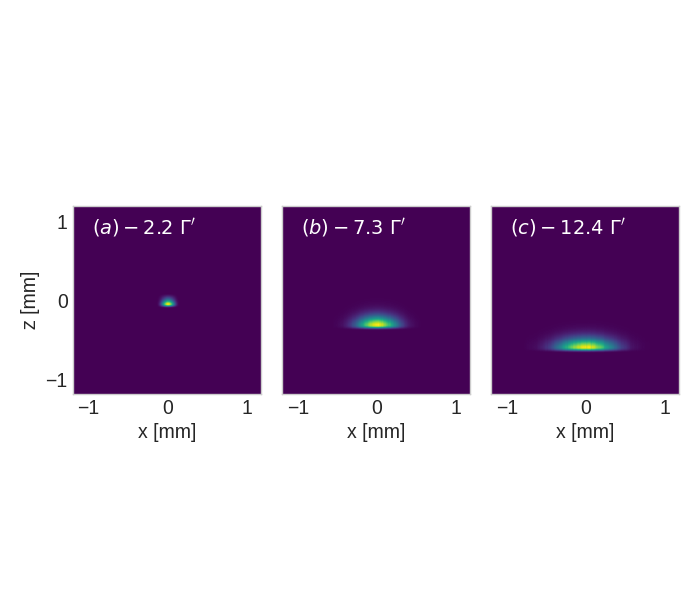
\includegraphics[width=0.9\textwidth]{USPSC-img/sr_loftus_cloud_profile.png}
    \vspace{5px}
    \legend{Simulated strontium cloud profile for three laser detunings: $ \delta = -5.0\Gamma' $ (a), $ \delta = -8.6\Gamma' $ (b), and $ \delta = -11.1\Gamma' $ (c), where $ \Gamma' = \Gamma \sqrt{1 + s_0} $ is the power-broadened linewidth. \\ Source: author}
    \label{fig:sr-loftus-atomic-cloud-profile}
\end{figure}

\begin{figure}[!ht]
    \centering
    \caption{Centre of mass of the ${}^{88}Sr$ nMOT as a function of the lasers detuning}
    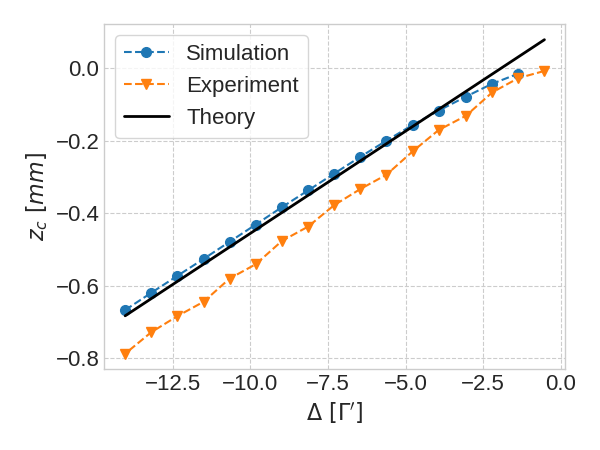
\includegraphics[width=0.6\textwidth]{USPSC-img/sr_centre_of_mass.png}
    \vspace{5px}
    \legend{centre of mass.\\ Source: author}
    \label{fig:sr-centre-of-mass}
\end{figure}

\begin{figure}[!ht]
    \centering
    \caption{Cloud size of the ${}^{88}Sr$ nMOT}
    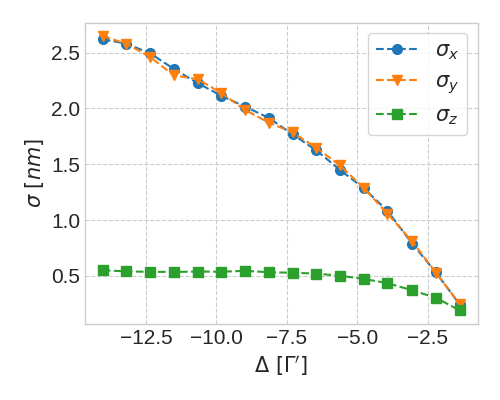
\includegraphics[width=0.8\textwidth]{USPSC-img/sr_loftus_cloud_size.png}
    \vspace{5px}
    \legend{cloud size.\\ Source: author}
    \label{fig:sr-loftus-cloud-size}
\end{figure}


%-----------------------------------
\subsection{Temperature}
\label{temperature}
%-----------------------------------

Experimental data from the \textit{strontium-ifsc}.

\begin{figure}[!ht]
    \centering
    \caption{Temperature of the ${}^{88}Sr$ nMOT as a function of the lasers detuning}
    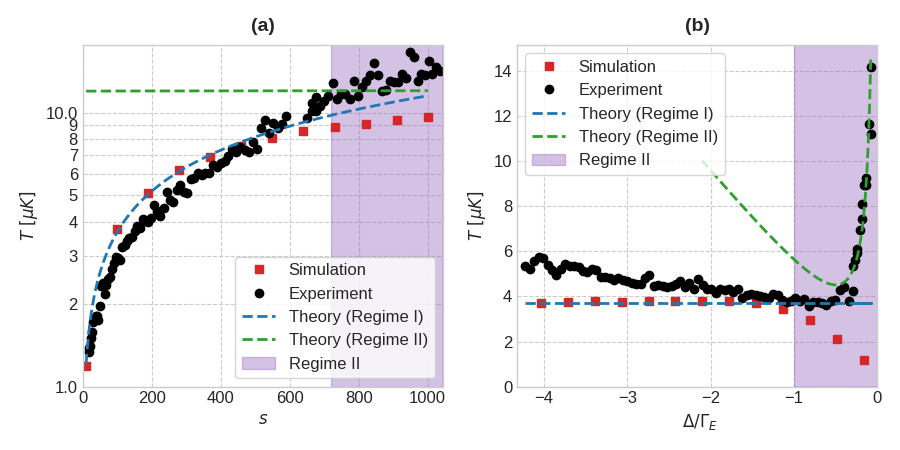
\includegraphics[width=1.0\textwidth]{USPSC-img/sr_temperature.png}
    \vspace{5px}
    \legend{temperature.\\ Source: author}
    \label{fig:sr-temperature}
\end{figure}
